\documentclass[12pt]{article}
% Include any special packages you might use.
\usepackage{amssymb,amsmath,amsthm,cool} %Provides extra symbols
\usepackage[height=9in,width=6.5in]{geometry} %Adjusts margins
\parindent=0pt % disables indentation
% The following commands set up the material that appears
% in the header.
\usepackage{fancyhdr}
\usepackage{parskip}
\usepackage{graphicx}
\lhead{\Huge{CS 241: HW8}} %change to section
%\chead{\today}  % Uncomment this line so add date to title

\rhead{Andrew Brandt} %Replace with your name
\pagestyle{fancy}
% If you want, you can make new commands, e.g. the following
\def\R{\mathbb R} %Define some commonly used symbols
\def\Q{\mathbb Q}
\def\Z{\mathbb Z}
\def\N{\mathbb N}

\title{CS 248 Unit 2 Homework 1}

\begin{document}

    \bf{1.}
    \begin{itemize}
        \item[a.] OR gates: 7432
        \item[b.] XOR gates: 7486 74386
        \item[c.] NOT gates: 7404
        \item[d.] NOR gates: 7402
        \item[e.] NAND gates: 7400, 7410, 7420
        \item[f.] D Flip Flops: 7473, 7473A, 7474, 74109, 74113
    \end{itemize}

    \bf{2.} Half Adder

        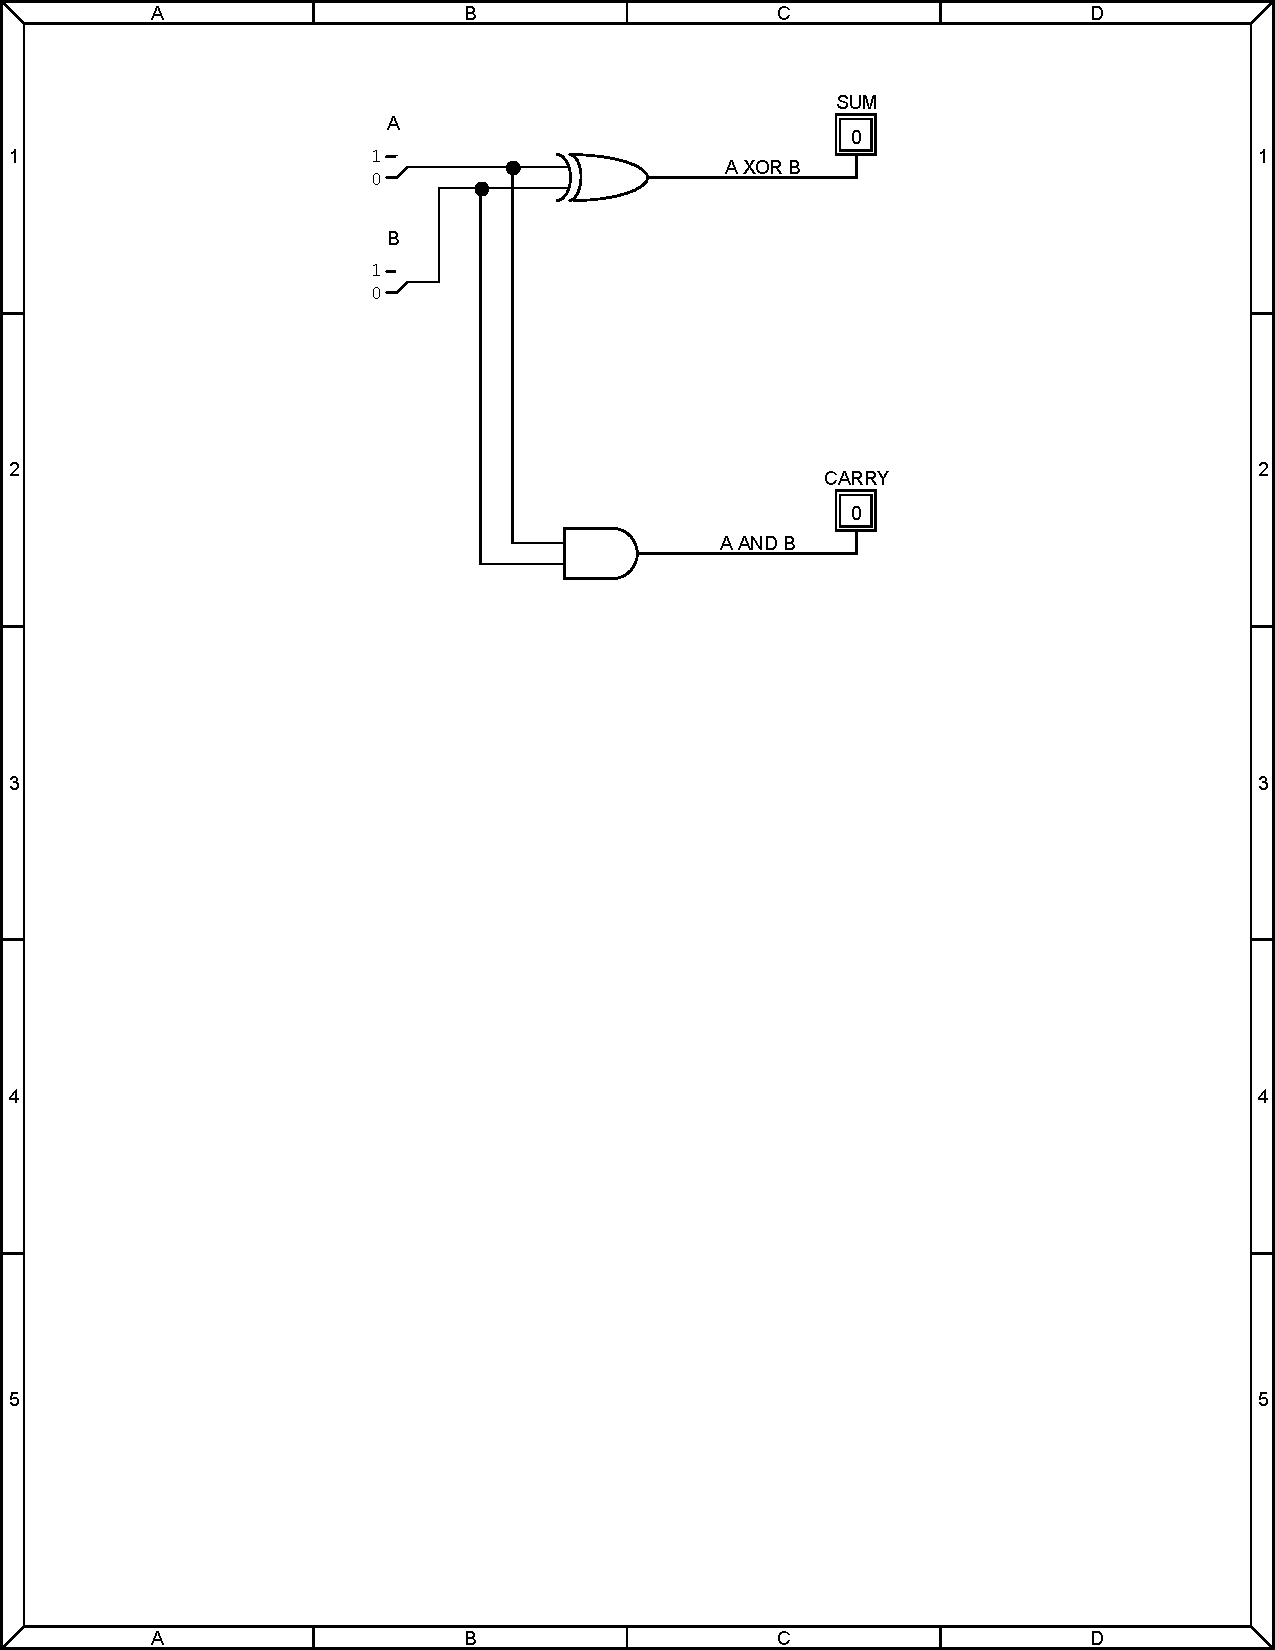
\includegraphics[scale=.5]{halfadderpdf}

    \bf{3.} Full Adder

        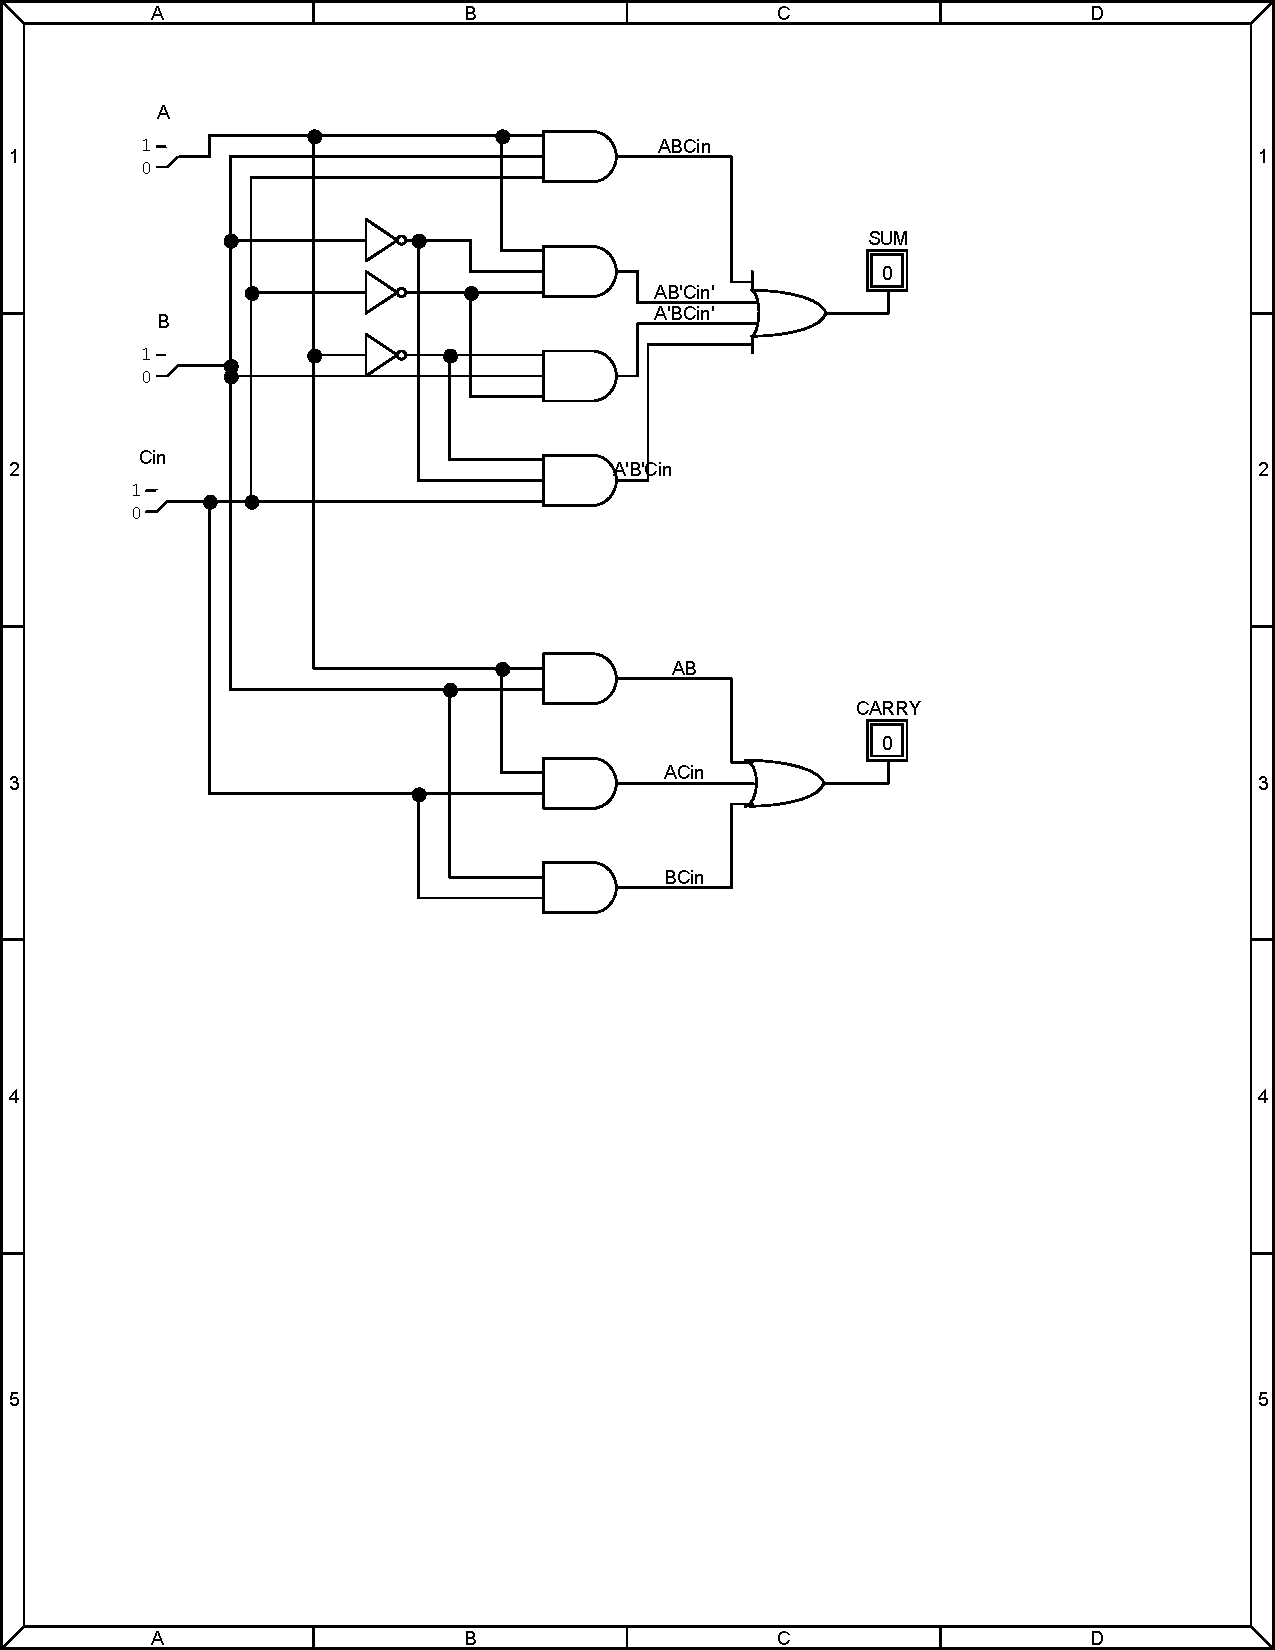
\includegraphics[scale=.5]{fulladderpdf}

    \bf{5.} 2 Bit Adder No IC 

        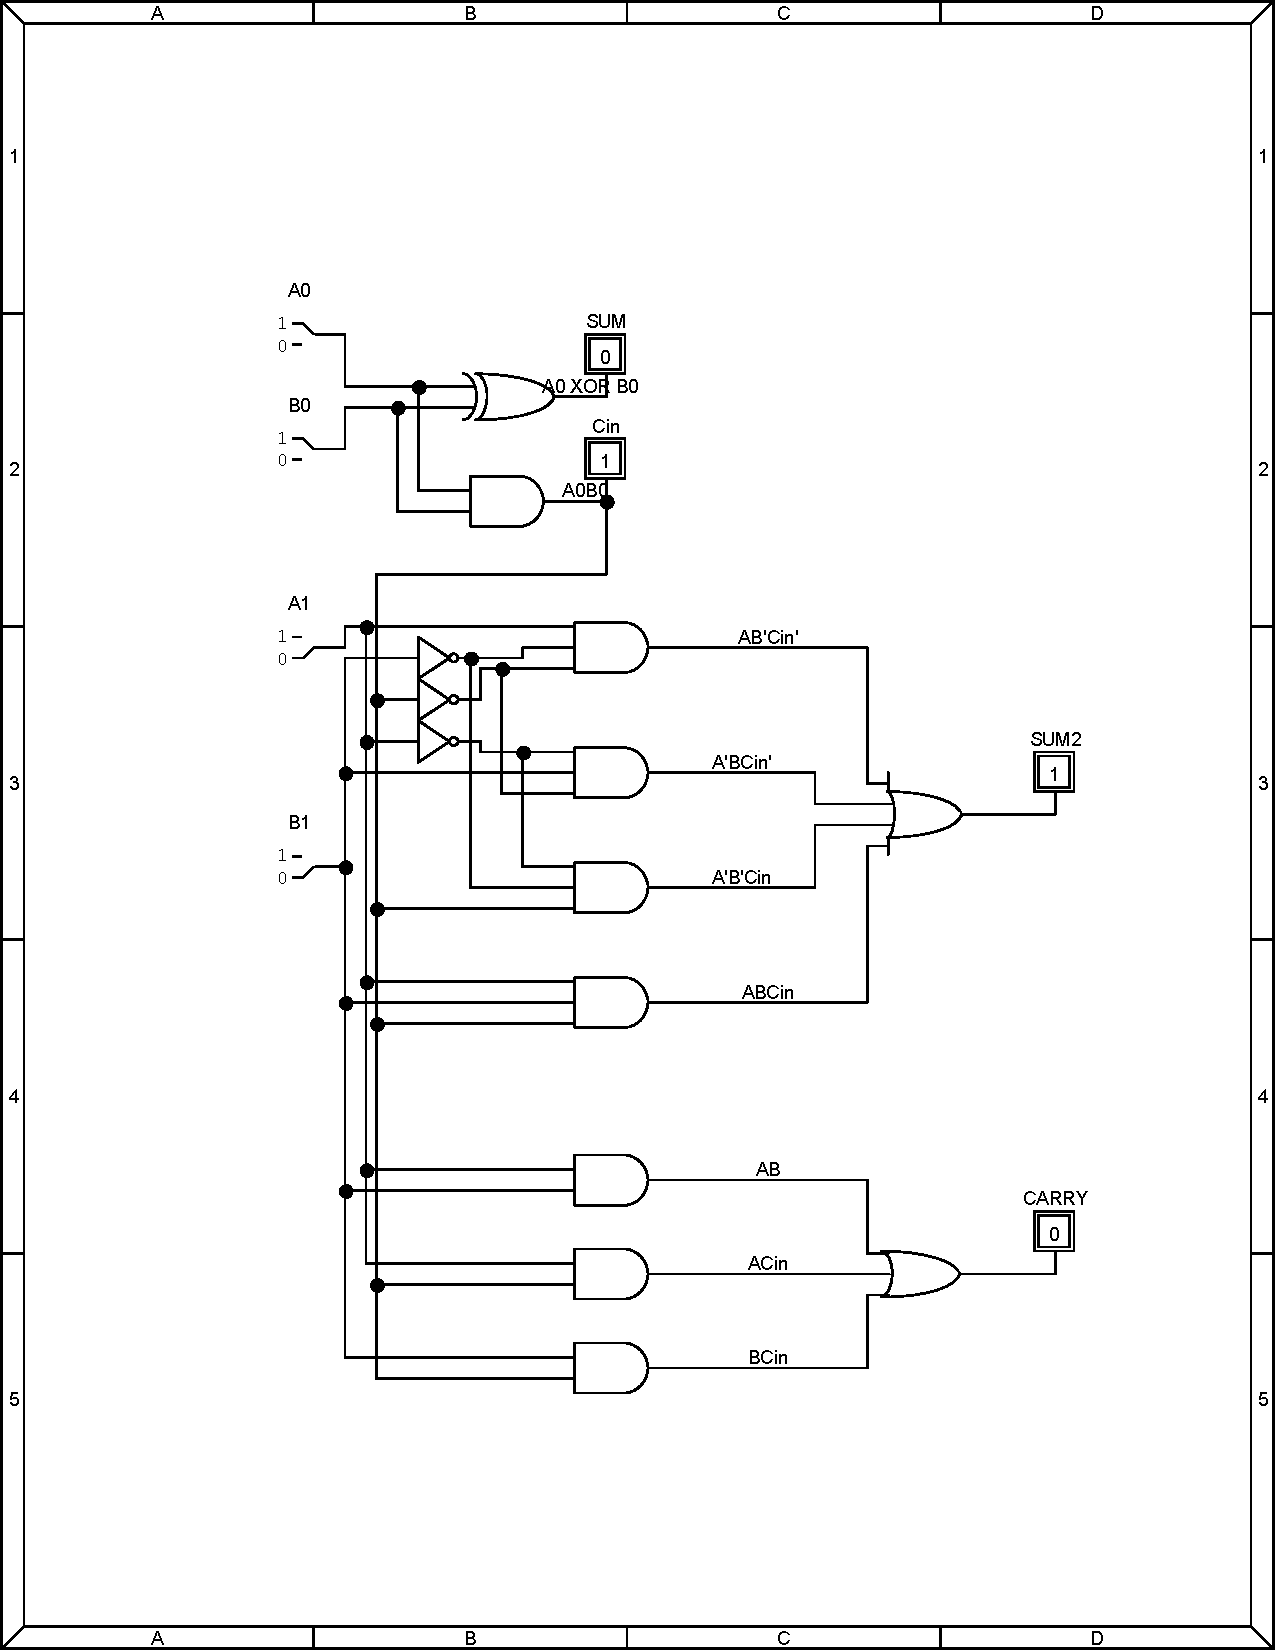
\includegraphics[scale=.5]{2bitadderpdfnoic}

    \bf{6.} 2 Bit Adder IC

        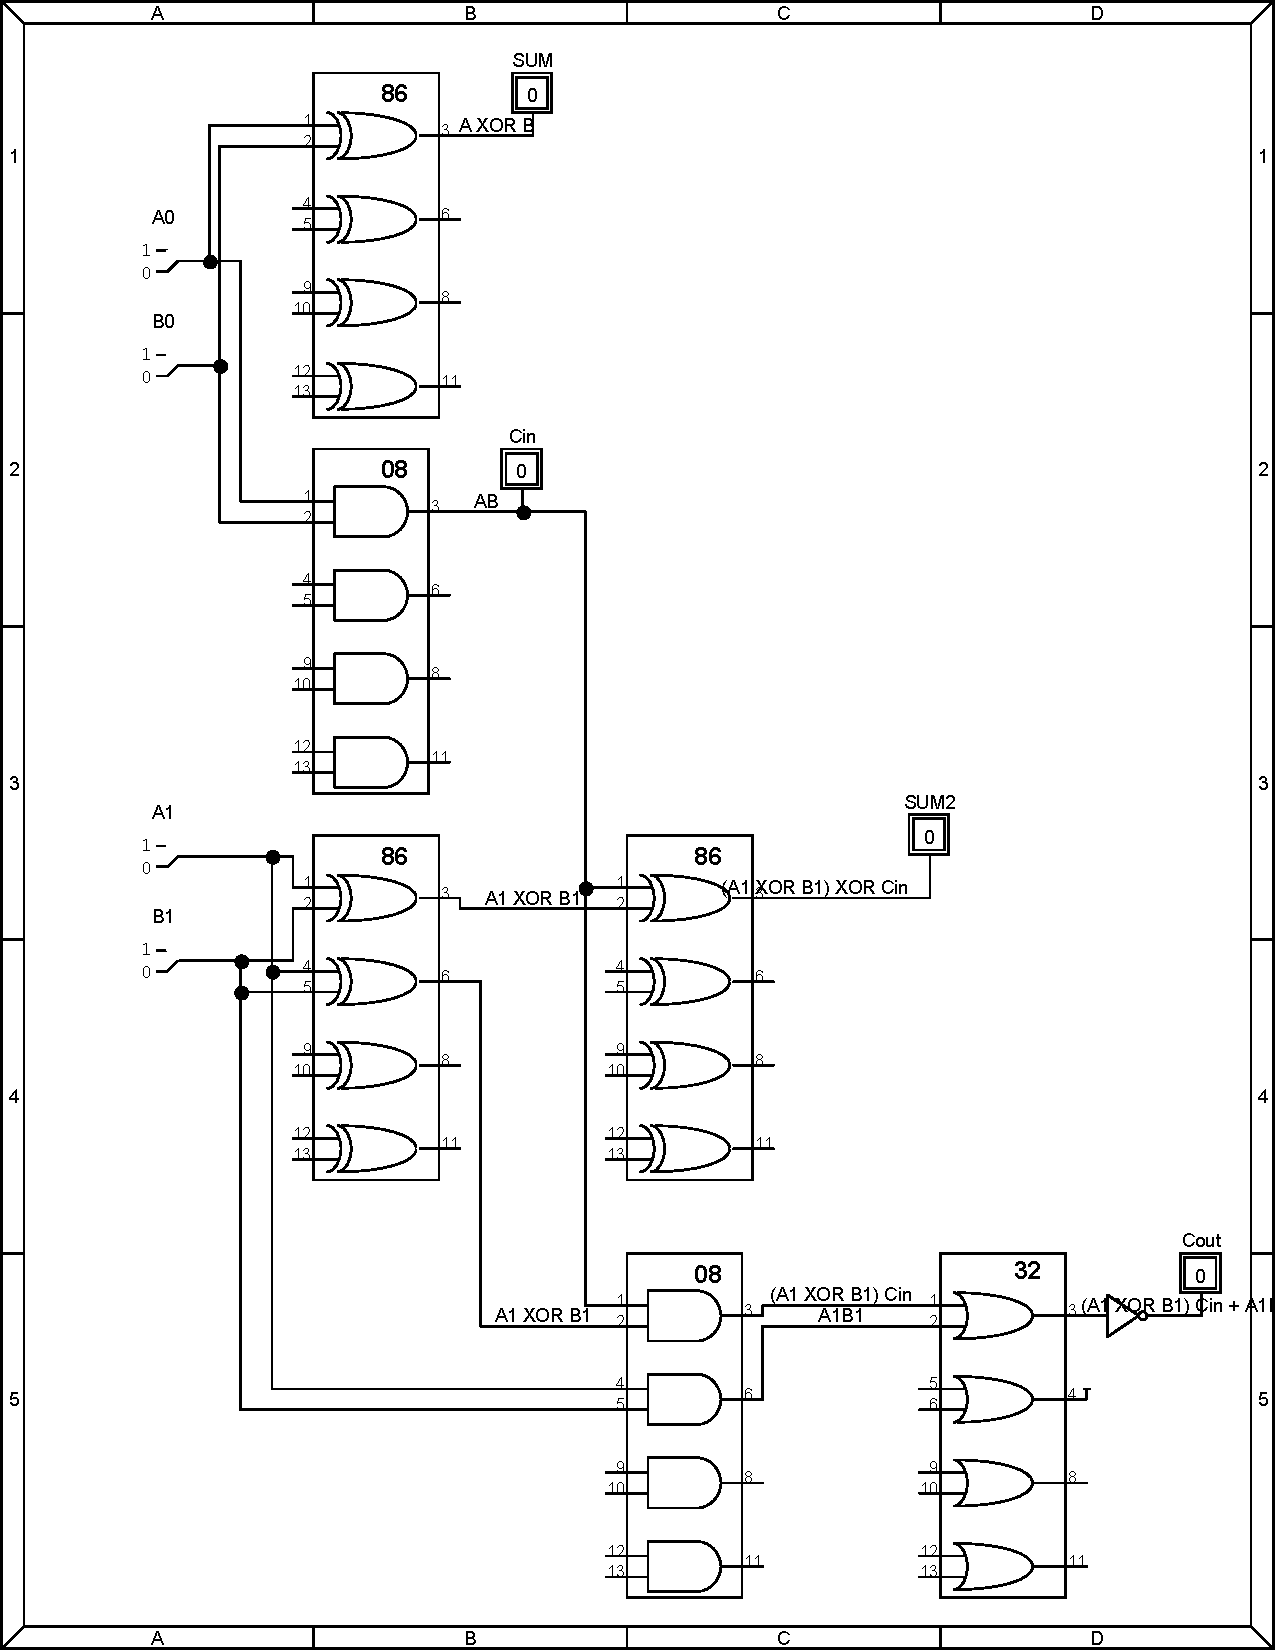
\includegraphics[scale=.5]{2bitadderpdfic}

\end{document}